\chapter{2次元共形場理論での2重分離クエンチ}\label{chap:doublequench}
この章では我々の研究\cite{Caputa:2019avh}に基づき、直線上の共形場理論の真空を2重分離クエンチしたときのエンタングルメントエントロピーの時間発展を調べる。\ref{sec:DSQsetup}節ではレプリカ法による計算のセットアップを説明し、\ref{sec:DSQdirac}節で零質量自由Dirac場での計算をする。\ref{sec:DSQholcft}節で重力双対を持つような2次元共形場理論でのエンタングルメントエントロピーの時間発展を計算する。そして最後に\ref{sec:DSQSPQ}で1重分離クエンチと2重分離クエンチの違いについて論じる。前章で論じた(1重)分離クエンチの重力側での対応物は、AdS時空に非常に``重い"障害を与えたが、2重分離クエンチの対応物となる障害は互いに重力相互作用によって近づくと予想できる。この予想を、測地線の長さを測る笠-高柳公式によって確認した。

\section{問題設定}\label{sec:DSQsetup}
2次元共形場理論における2重分離クエンチとは、空間方向の異なる2点での相互作用を時刻$t=0$で瞬時に同時に``切る''ことを指す。切られた部分を境界として、分離によって因果的に独立な3つの領域$L,C,R$が生じる(図\ref{fig:dqlorentz})。
\begin{figure}[h]
	\centering
	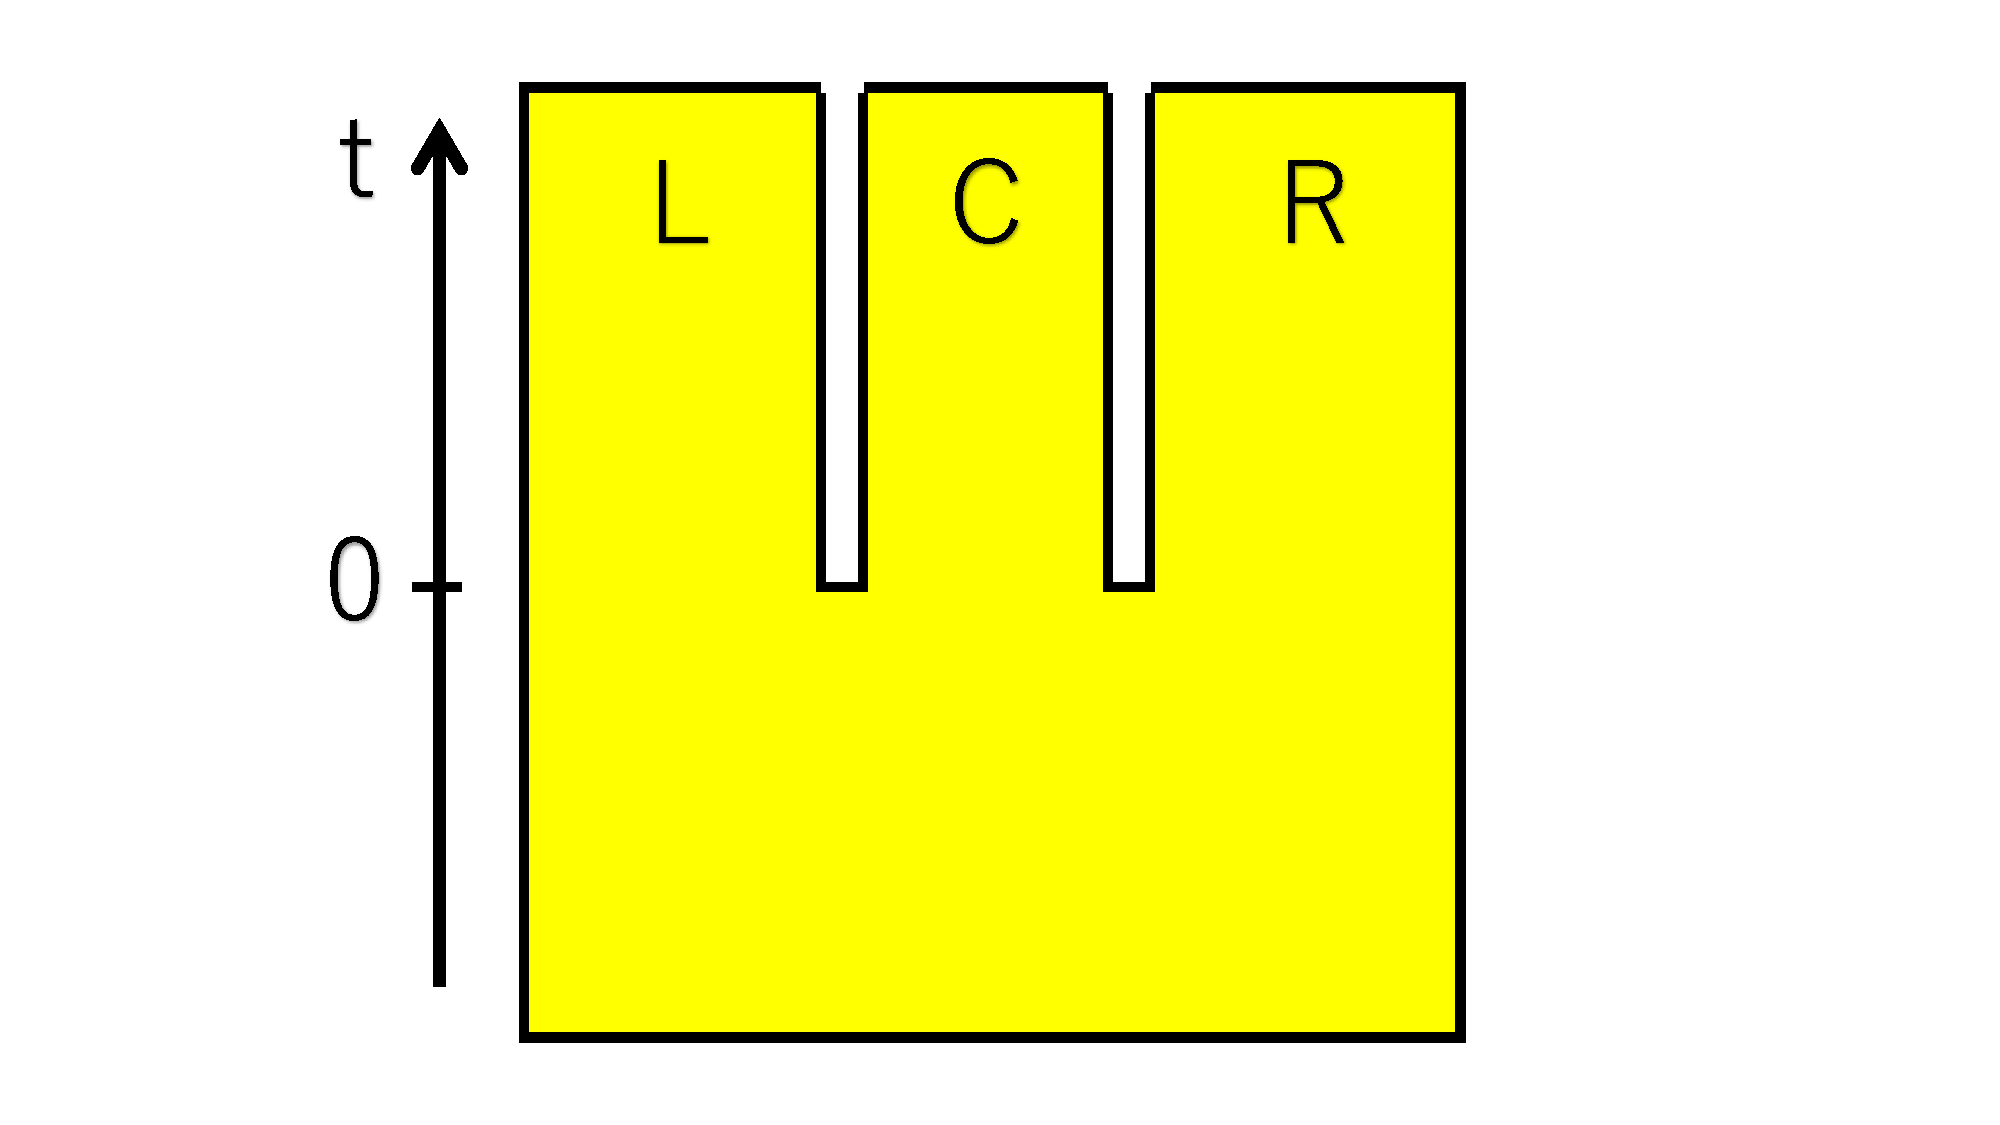
\includegraphics[width=0.7\linewidth]{DQlorentz.pdf}
	\label{fig:dqlorentz}
	\caption{2重分離クエンチされた系の図。分離によって因果的に独立な3つの領域$L,C,R$が生じる。}
\end{figure}

真空を分離クエンチした状態に対するエンタングルメントエントロピーをレプリカ法で計算するには、虚時間$\tau=-0,+0$面にクエンチされた状態$|\Psi\ra, \la\Psi|$を経路積分で用意して、注目系以外をトレースアウトしてorbifoldを作る。そして、実時間でのエンタングルメントエントロピーを得るには、レプリカ法で得た虚時間のエンタングルメントエントロピーの結果を$\tau\to 0+it$と解析接続する。

虚時間でのセットアップは$[\pm b-ia,\pm b+ia]$を2つの分離の境界とし図\ref{fig:dqmapping}で表される。これは
\begin{align}
w(\nu)&=x+i\tau=b\left( 1+ K_{\beta^{-1}}(\nu)+K_{\beta^{-1}}\left(\nu+\frac{i\beta^{-1}}{2}\right) \right)\\
K_{\beta^{-1}}(\nu)&=\frac{1}{\pi i}\left.\frac{\del}{\del \nu'}\log\theta_1(\nu',i\beta^{-1})\right|_{\nu'=\nu}
\end{align}
とすることで、$\IM \nu=\pm \beta^{-1}/4$に境界をもち、$\nu\sim \nu+1$と同一視の入った円筒に移る\cite{sakajo2012force}\cite{Numasawa_2016}。
\begin{figure}[h]
	\centering
	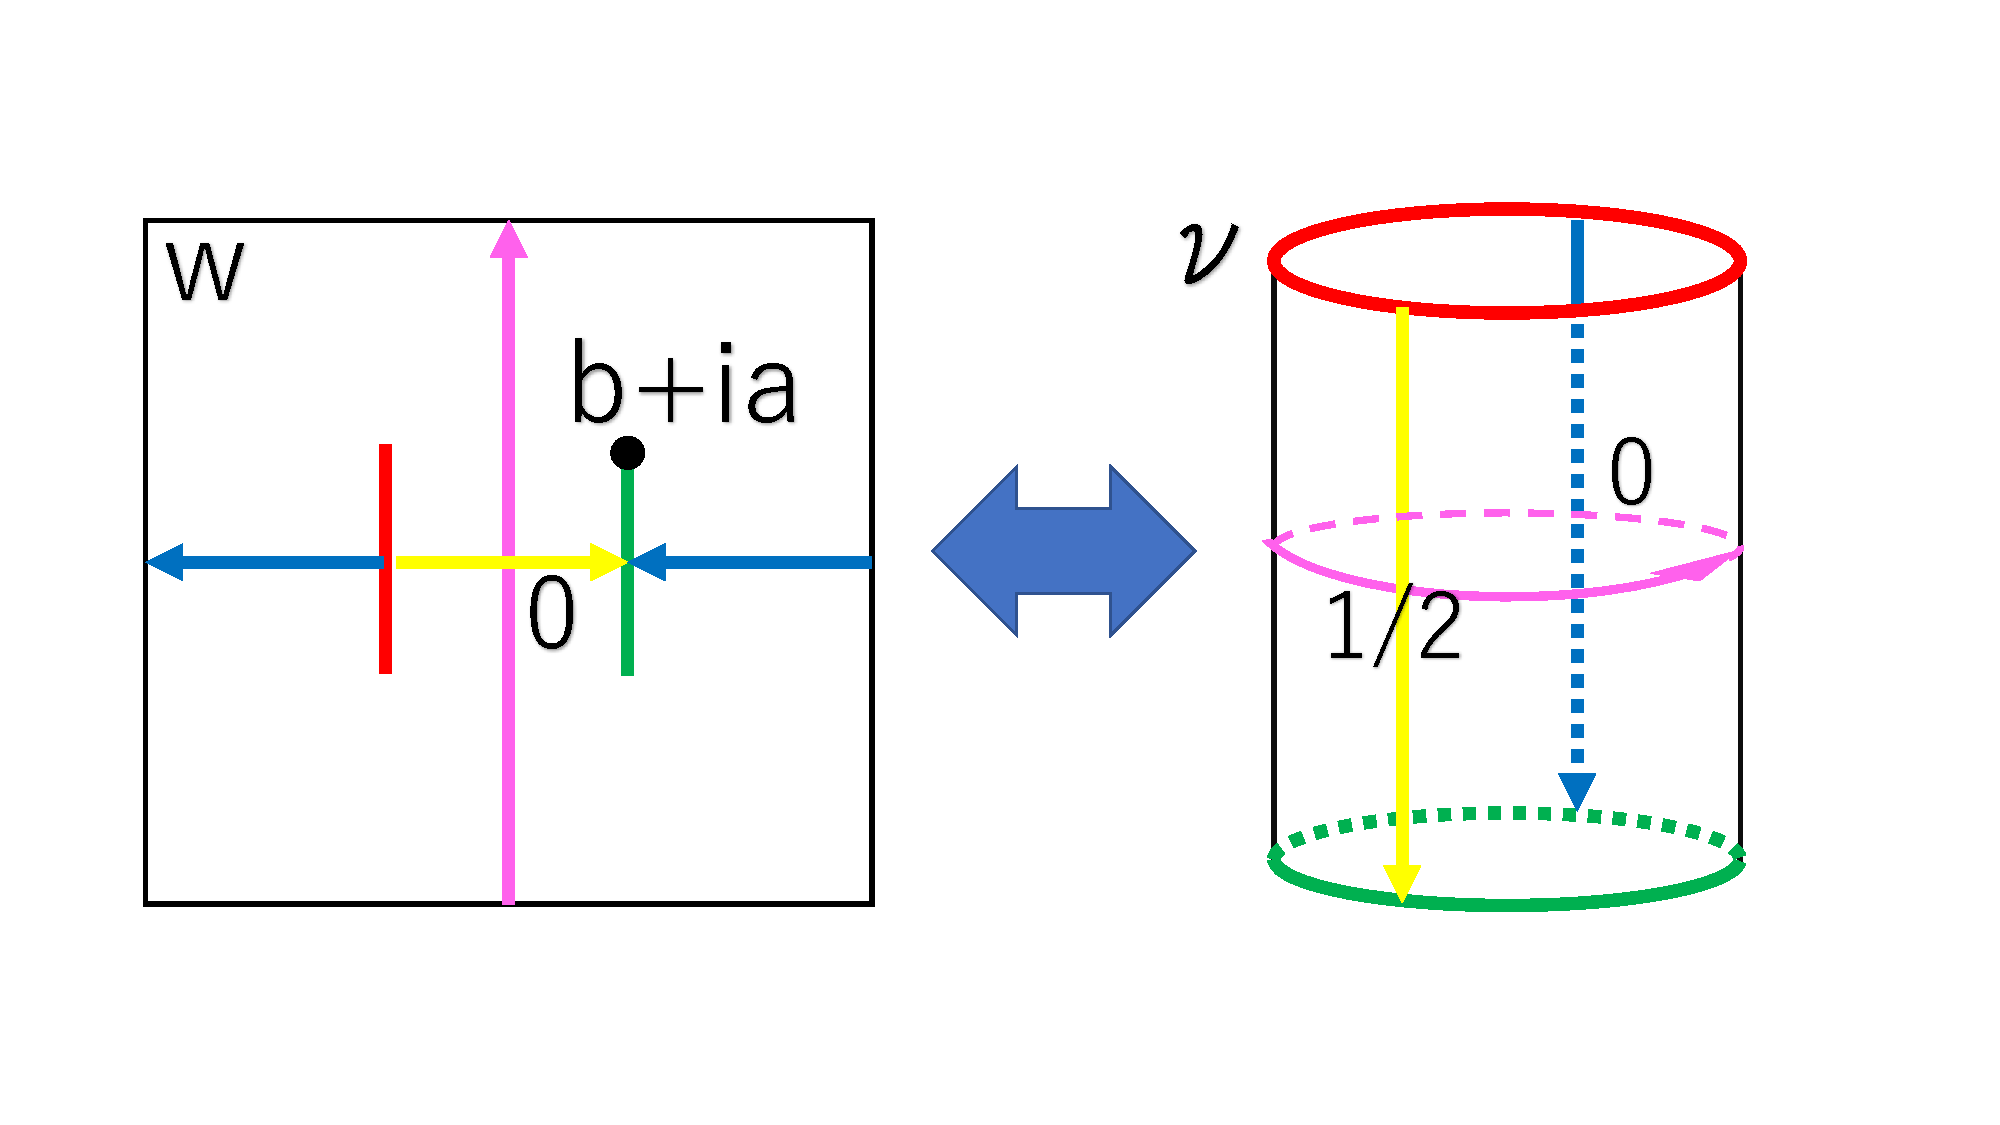
\includegraphics[width=0.7\linewidth]{DQmapping.pdf}
	\label{fig:dqmapping}
	\caption{左は2重分離クエンチされた真空についてのレプリカ法のセットアップの図。これを共形変換することで右図の有限長さの円筒に移る。}
\end{figure}

この円筒は
\begin{align}
2\pi i \beta\nu = \zeta
\end{align}
とすることで、$\RE \zeta=\pm \pi/2$に境界をもち、$\zeta\sim \zeta+2\pi i \beta$と同一視の入った円筒に移る。このとき複素共役は$\overline{w(\zeta)}=w(\overline{\zeta})$で関係づいていることに注意しておく。

パラメータ$\beta^{-1}$は$a/b$のみで決定され、その関係は次のようなグラフになる。
\begin{figure}[h]
	\centering
	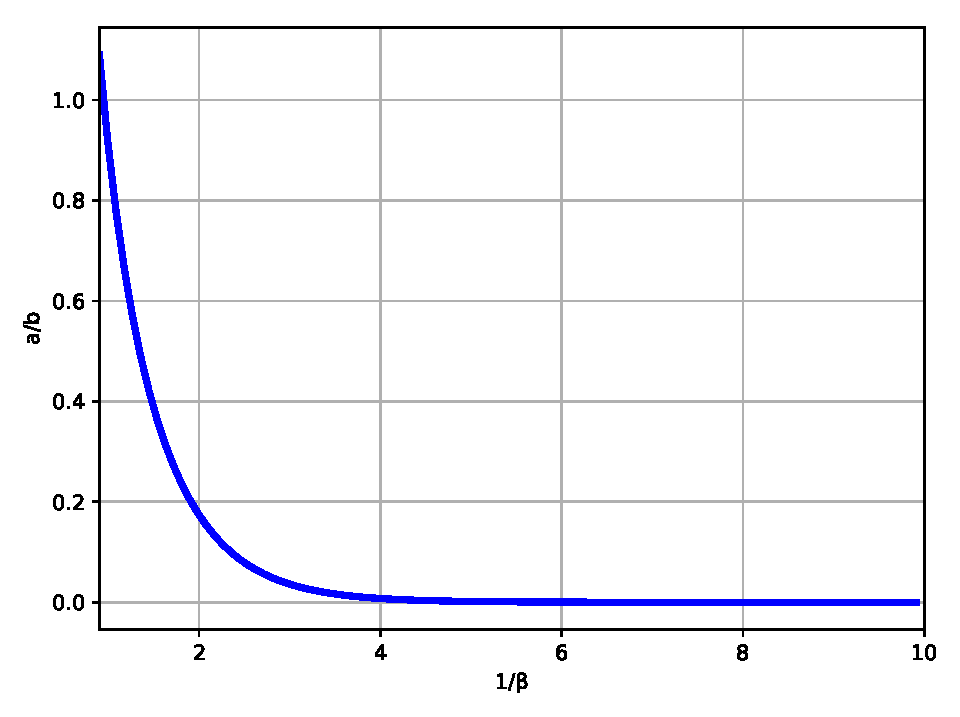
\includegraphics[width=0.5\linewidth]{s2aoverb.pdf}
	\caption{$b=50$に固定したときの、横軸が$\beta^{-1}$で縦軸が$a/b$のグラフ}
\end{figure}

$\beta^{-1}$と$a/b$の関係は、テータ関数の高温・低温極限の近似式から、$a/b\to 0,\infty$の極限で
\begin{align}
\beta^{-1}\sim \left\{ \begin{array}{ll}
\bigskip \dfrac{2b}{a} & (a/b\to \infty\iff \beta^{-1}\to 0)\\
\dfrac{2}{\pi}\log\dfrac{4b}{a} & (a/b\to 0\iff \beta^{-1}\to \infty)
\end{array}\right.
\end{align}
と近似できる。

\section{自由Dirac場}\label{sec:DSQdirac}
\subsection{EEの時間発展}
\subsub{解析計算}
$2$つの区間$[\pm b-ia,\pm b+ia]$での境界条件としてともにNeumann境界条件を課す。また、$\RE \nu$方向が$w$座標での時間方向に対応していることから、$\nu\sim \nu+1$の周期に対してNSセクターのDirac場を考える。

\ref{chap:adscftreview}章での頂点演算子の円筒$2$点関数を$\nu$座標での境界の取り方に合わせて読み替えると、零質量自由Dirac場の真空のエンタングルメントエントロピーは
\begin{align}
S_A &=\frac{1}{6}\log(\frac{G}{\epsilon^2})\\
G&=\frac{1}{(2\pi)^2}\left|\frac{dw_1}{d\nu_1}\right|\left|\frac{dw_2}{d\nu_2}\right|\notag\\
&\times \frac{\theta_1\left(\nu_1-\nu_2|i\beta^{-1}\right)\theta_1
	\left(\overline{\nu}_1-\overline{\nu}_2|i\beta^{-1}\right)\theta_1\left(\nu_1-\overline{\nu}_1+\frac{i\beta^{-1}}{2}|i\beta^{-1}\right)\theta_1\left(\nu_2-\overline{\nu}_2+\frac{i\beta^{-1}}{2}|i\beta^{-1}\right)}{\eta(i\beta^{-1})^6 \theta_1\left(\nu_1-\overline{\nu}_2+\frac{i\beta^{-1}}{2}|i\beta^{-1}\right)\theta_1
	\left(\nu_2-\overline{\nu}_1+\frac{i\beta^{-1}}{2}|i\beta^{-1}\right)}
\end{align}
となる。$2\pi i\beta \nu=\zeta$の座標変換(モジュラー変換)を用いれば、上のエンタングルメントエントロピーは\ref{fincylvertex2ptfunc}の相関関数の式をそのまま使って書くことができる。しかしいま興味のある場合は$a/b\to 0 \iff \beta\to 0$の``高温極限"の場合であるから、$\zeta$座標での相関関数を使うと数値計算でのテータ関数の収束性が悪くなる。そこで今回は$\nu$座標での相関関数を使っている。

\subsub{数値計算}
真空の寄与を引いたEE $S_A(t)-S_\text{vac}$を数値計算したものがグラフ\ref{fig:dd528}である。$b=50,a\sim 0.05\iff \beta^{-1}=5.28$で計算しており、左上図は部分系$[100,200]$、右上図は部分系$[10,30]$、左下図は部分系$[30,100]$、右下図は$[-150,100]$にとった場合である。
\begin{figure}[H]
	\centering
	\begin{tabular}{c}
		\begin{minipage}{0.50\hsize}
			\centering
			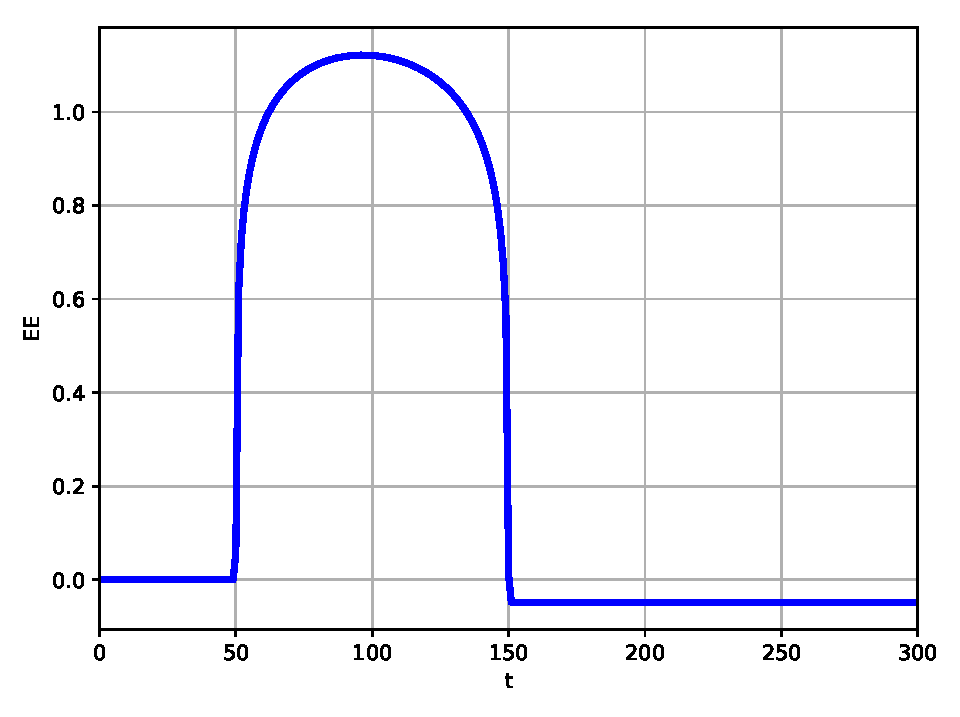
\includegraphics[width=\linewidth]{dd528_100_200.pdf}
		\end{minipage}
		\begin{minipage}{0.50\hsize}
			\centering
			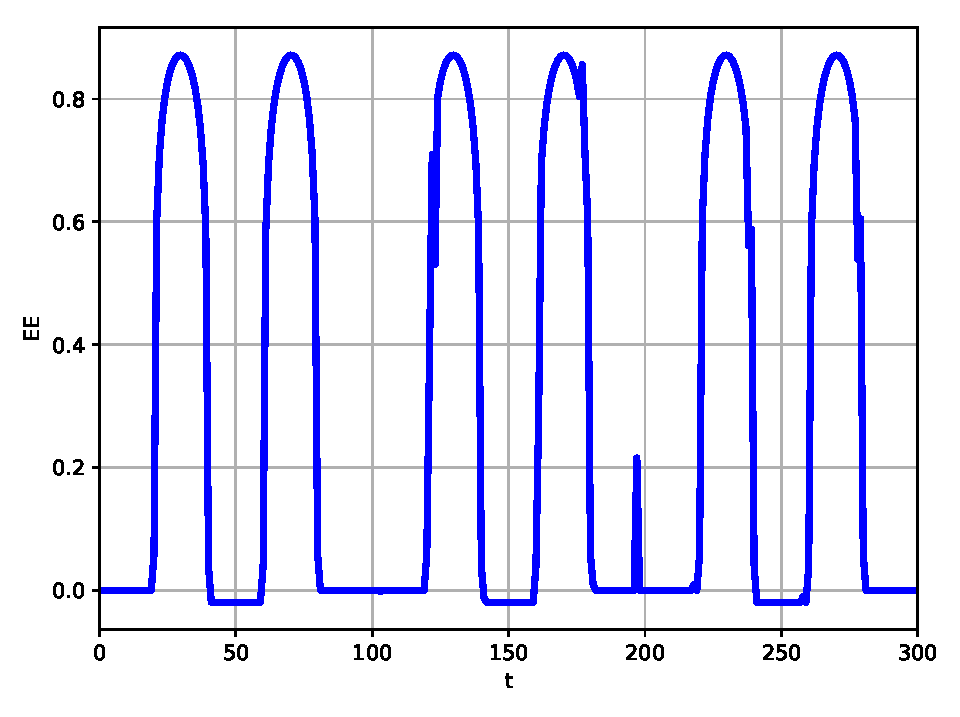
\includegraphics[width=\linewidth]{dd528_10_30.pdf}
		\end{minipage}
		\begin{minipage}{0.06\hsize}
			\vspace{10mm}
		\end{minipage} \\
		\begin{minipage}{0.50\hsize}
			\centering
			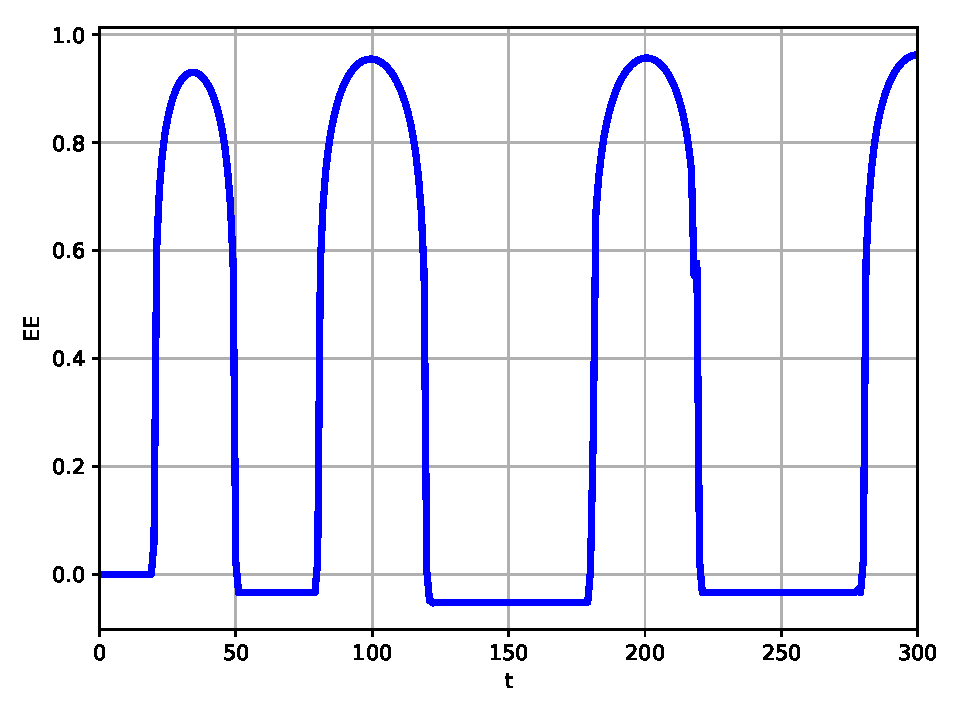
\includegraphics[width=\linewidth]{dd528_30_100.pdf}
		\end{minipage}
		\begin{minipage}{0.50\hsize}
			\centering
			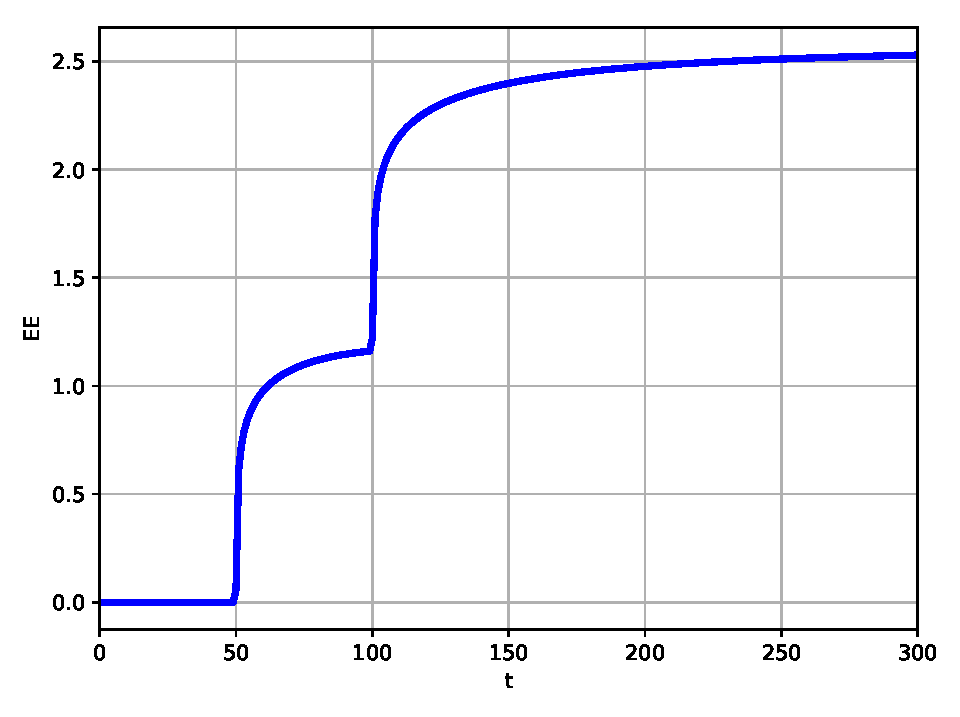
\includegraphics[width=\linewidth]{dd528_150_100.pdf}
		\end{minipage}
	\end{tabular}
	\caption{自由Dirac場の真空を$b=50,a\sim 0.05$で2重分離クエンチしたときのEEのグラフ。横軸は時間$t$で、縦軸は真空の寄与を引いたEE $S_A(t)-S_\text{vac}$をプロットしている。}
	\label{fig:dd528}
\end{figure}

次に$b=50,a\sim 50 \iff \beta^{-1}=0.945$で計算した結果をグラフ\ref{fig:dd0945}にあげる。部分系の取り方は同様で、左上図は部分系$[100,200]$、右上図は部分系$[10,30]$、左下図は部分系$[30,100]$、右下図は$[-150,100]$にとった場合である。
\begin{figure}[H]
	\centering
	\begin{tabular}{c}
		\begin{minipage}{0.50\hsize}
			\centering
			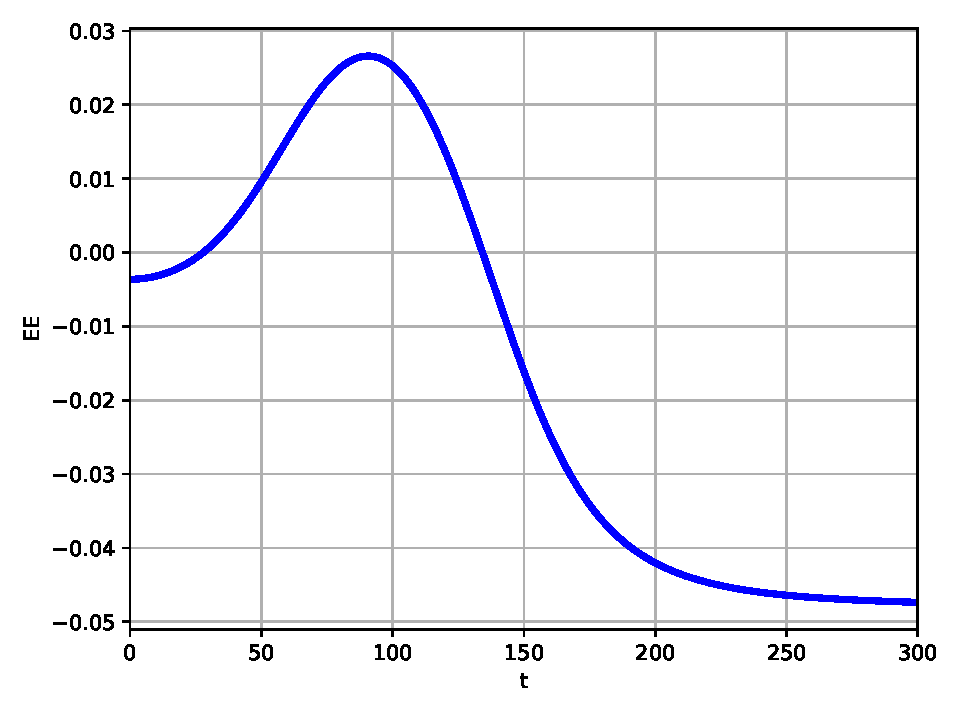
\includegraphics[width=\linewidth]{dd0945_100_200.pdf}
		\end{minipage}
		\begin{minipage}{0.50\hsize}
			\centering
			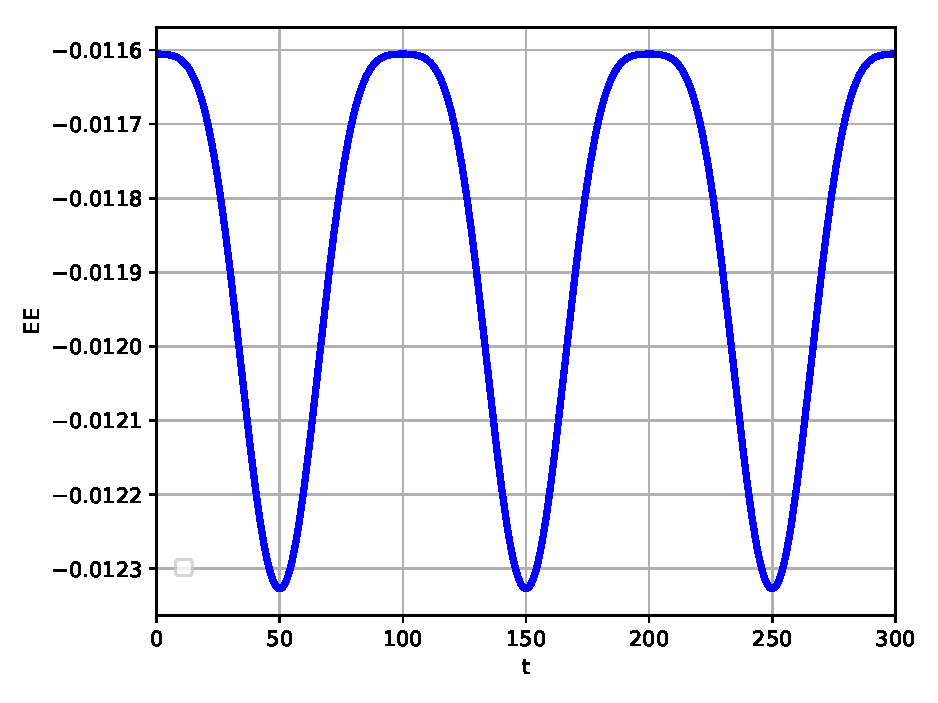
\includegraphics[width=\linewidth]{dd0945_10_30.pdf}
		\end{minipage}
		\begin{minipage}{0.06\hsize}
			\vspace{10mm}
		\end{minipage} \\
		\begin{minipage}{0.50\hsize}
			\centering
			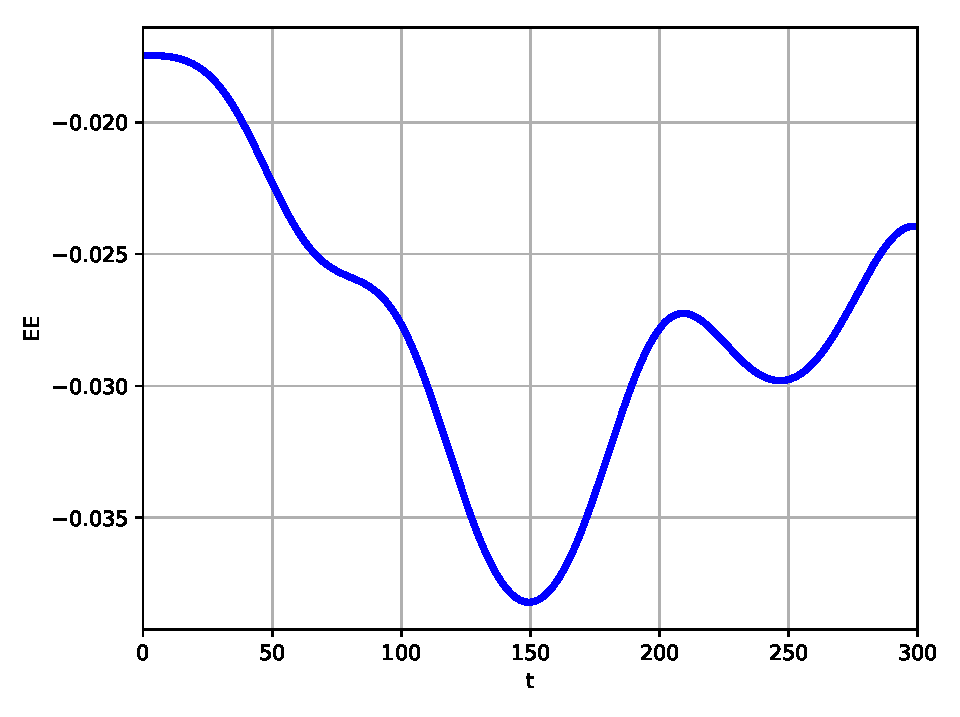
\includegraphics[width=\linewidth]{dd0945_30_100.pdf}
		\end{minipage}
		\begin{minipage}{0.50\hsize}
			\centering
			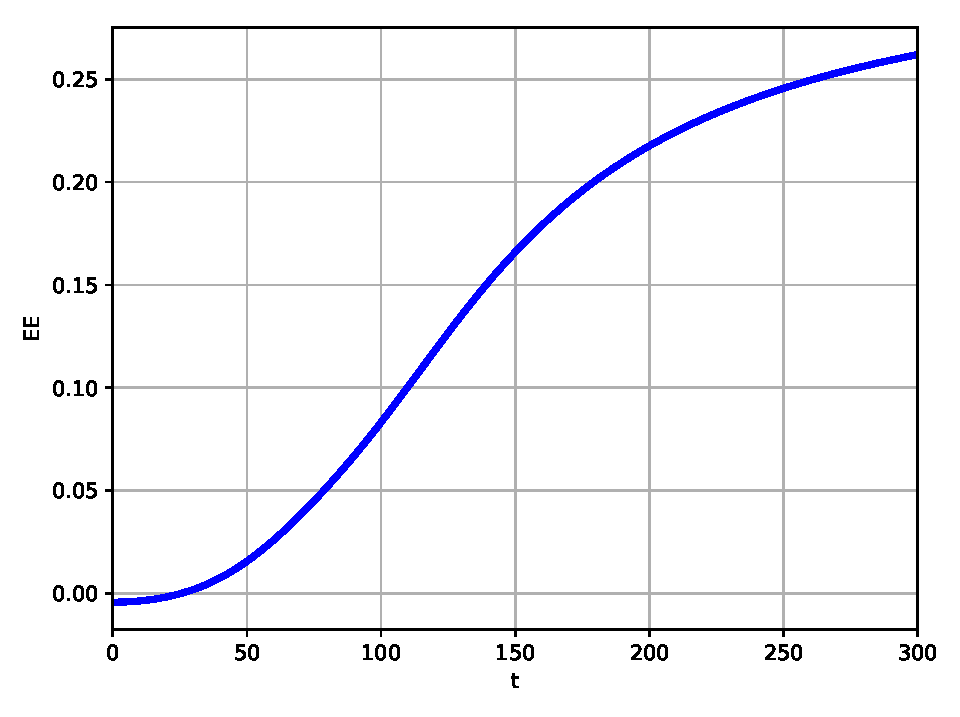
\includegraphics[width=\linewidth]{dd0945_150_100.pdf}
		\end{minipage}
	\end{tabular}
	\caption{自由Dirac場の真空を$b=50,a\sim 50$で2重分離クエンチしたときのEEのグラフ。横軸は時間$t$で、縦軸は真空の寄与を引いたEE $S_A(t)-S_\text{vac}$をプロットしている。}
	\label{fig:dd0945}
\end{figure}
いずれの結果も右下の図を除いて、準粒子描像に当てはまっていることが分かる。

\subsection{中央の領域の熱力学的エントロピー}
\subsub{中央の領域の熱力学的エントロピー}
2重分離クエンチを考えると空間領域は$L,C,R$の$3$つに分かれる。円筒分配関数\ref{diracPFfincyl}から中央の領域の$t\to\infty$における熱力学的エントロピーを求める。エンタングルメントエントロピーの計算に用いたのは$\nu$座標での相関関数だったから、
\begin{align}
\log Z(\beta) &= \log \frac{\theta_3(0|i\beta^{-1})}{\eta(i\beta^{-1})}\\ &=\frac{\pi\beta^{-1}}{12}+2\sum_{m=1}^{\infty}\log (1+e^{-2\pi(m-\frac{1}{2})\beta^{-1}})
\end{align}
であることに注意すると、熱力学的エントロピーは
\begin{align}
S_\text{thermal}&=-\frac{\del \left(-(2\pi\beta)^{-1}\log Z(\beta)\right)}{\del (2\pi\beta)^{-1}}\\
&=\frac{1}{6}\pi\beta^{-1}+2\sum_{m=1}^{\infty} \log(1+e^{-2\pi (m-1/2)\beta^{-1}})-4\pi\beta^{-1}\sum_{m=1}^{\infty}\frac{m-1/2}{1+e^{2\pi (m-1/2)\beta^{-1}}}
\end{align}
となる。さらに$\beta\to 0$の高温極限で熱力学的エントロピーは
\begin{align}
S_\text{thermal}\sim \frac{1}{6}\pi\beta^{-1}\sim \frac{1}{3}\log\frac{4b}{a}
\end{align}
となる。これはBTZブラックホールのエントロピー$\frac{c}{3}\pi\beta^{-1}$を$1/2$倍したものと同じ形をしていることに注意しておく。また、$\beta\to 0$の極限は$b\gg a$の極限に等価である。したがって$S_\text{thermal}$は$a/2$を紫外カットオフと思ったときの領域$C$の真空のエンタングルメントエントロピーに一致することにも注意しておく。

\subsub{領域$L,R$に端点をもち、$C$にまたがるような大きな部分系$A$のEE}
部分系$A=[-X,X],\ X\gg b$のEEについて考える。部分系$A$を$(A\intersection L)\union C \union (A\intersection R)$と3つの因果的に独立な領域に分けると、領域$(A\intersection L),(A\intersection R)$は領域$C$に比べて非常に大きい。このとき領域$C$で起きたクエンチの情報は粗視化されてしまい、$C$は内部の情報にアクセスできなくなった領域として振る舞うようになると考えられる。また、領域$C$が小さい場合を考えるので、$a/b$も小さくなる($\iff$ 高温極限$\beta\to 0$)。したがって、$A$のEEは
\begin{align}
S_A&\sim (A\text{の真空のEE})+(C\text{の熱力学的エントロピー})\\
&=\frac{1}{3}\log\frac{2X}{\epsilon}+\frac{1}{6}\pi\beta^{-1}\label{thermalization}
\end{align}
となると推測される。

実際これが成り立つことを、数値計算で確かめてみる。$b=50,a\sim 0.05\iff \beta^{-1}=5.28$として、部分系$A=[-X,X]$の端点$X$を$100\le X \le 10000$まで変化させ、それぞれの系に対して$t=10^6$でのEE $S_A(t)-S_\text{vac}$を数値計算したものが図\ref{fig:cthermalization}である。
\begin{figure}[H]
	\centering
	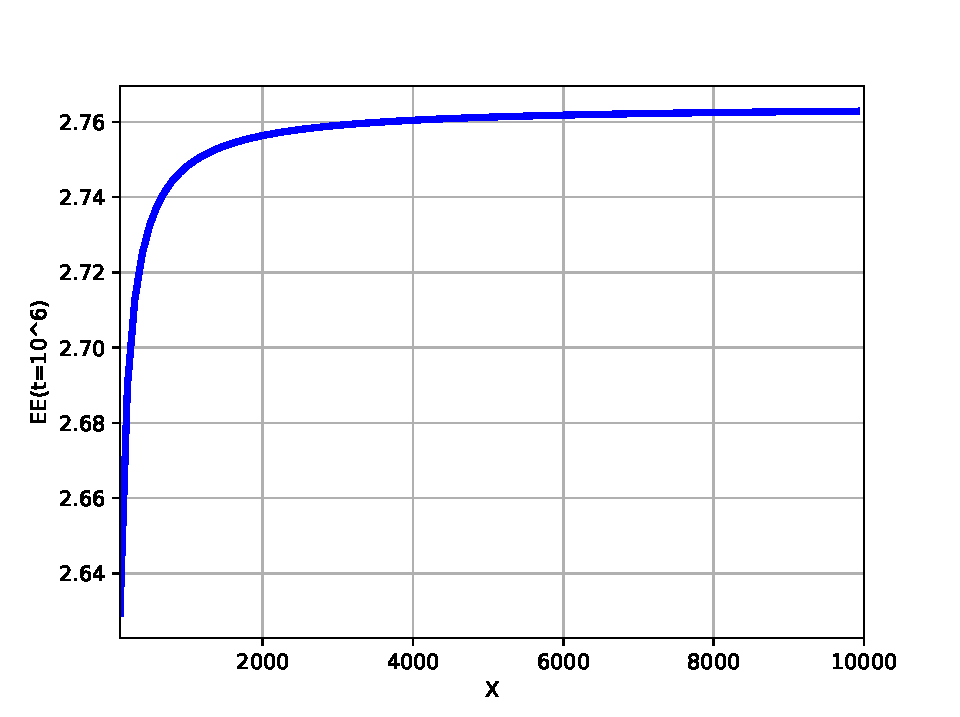
\includegraphics[width=0.7\linewidth]{Cthermalization.pdf}
	\caption{自由Dirac場の真空を$b=50,a\sim 0.05\iff \beta^{-1}=5.28$で2重分離クエンチしたときの、時刻$t=10^6$でのEEのグラフ。横軸は部分系の大きさ$X$で、縦軸は真空の寄与を引いたEE $S_A(t=10^6)-S_\text{vac}$をプロットしている。}
	\label{fig:cthermalization}
\end{figure}

このときたしかに$X\gg b$の``熱力学極限''で、真空の寄与を引いたEE $S_A(t)-S_\text{vac}$が領域$C$の熱力学的エントロピー
\begin{align}
S_\text{thermal}\sim \frac{1}{6}\pi\beta^{-1}\sim 2.76460\cdots
\end{align}
に漸近していて、(\ref{thermalization})が成立している。
\pagebreak
\section{重力双対をもつ共形場理論}\label{sec:DSQholcft}
重力双対をもつ、有限長さの円筒上の共形場理論に双対となるAdS空間を考えたい。

AdS/BCFTでNeumann境界条件を課せば、トーラスを境界に持つAdS空間であるthermal AdSやthermal non-rotating BTZが双対なAdS空間となる。どちらが双対な時空となるかはCFTの逆温度$\beta$で決まり、
\begin{align}
\beta<1 &\to \text{thermal non-rotating BTZ black hole}\\
\beta>1 &\to \text{thermal AdS}
\end{align}
で対応している。以下ではこの2つの場合に分けてエンタングルメントエントロピーを計算する。

\subsection{thermal non-rotating BTZ ($\beta<1$)の場合}
\subsub{解析計算}
$2\pi i \beta \nu=\zeta=X+i T$とすれば、$\zeta$座標の円筒にその鏡像を加えて得られるトーラスは
\begin{align}
X\sim X+2\pi,\ T\sim T+2\pi\beta
\end{align}
の同一視で作られる。(\ref{BTZblackbrane})より、このCFTに対応するthermal non-rotating BTZ計量は
\begin{align}
ds^2=\frac{R_A^2}{z^2}\left( \frac{dz^2}{1-z^2/\beta^2}+\left(1-z^2/\beta^2\right)dT^2+dX^2 \right)
\end{align}
となる。
\begin{figure}[h]
	\centering
	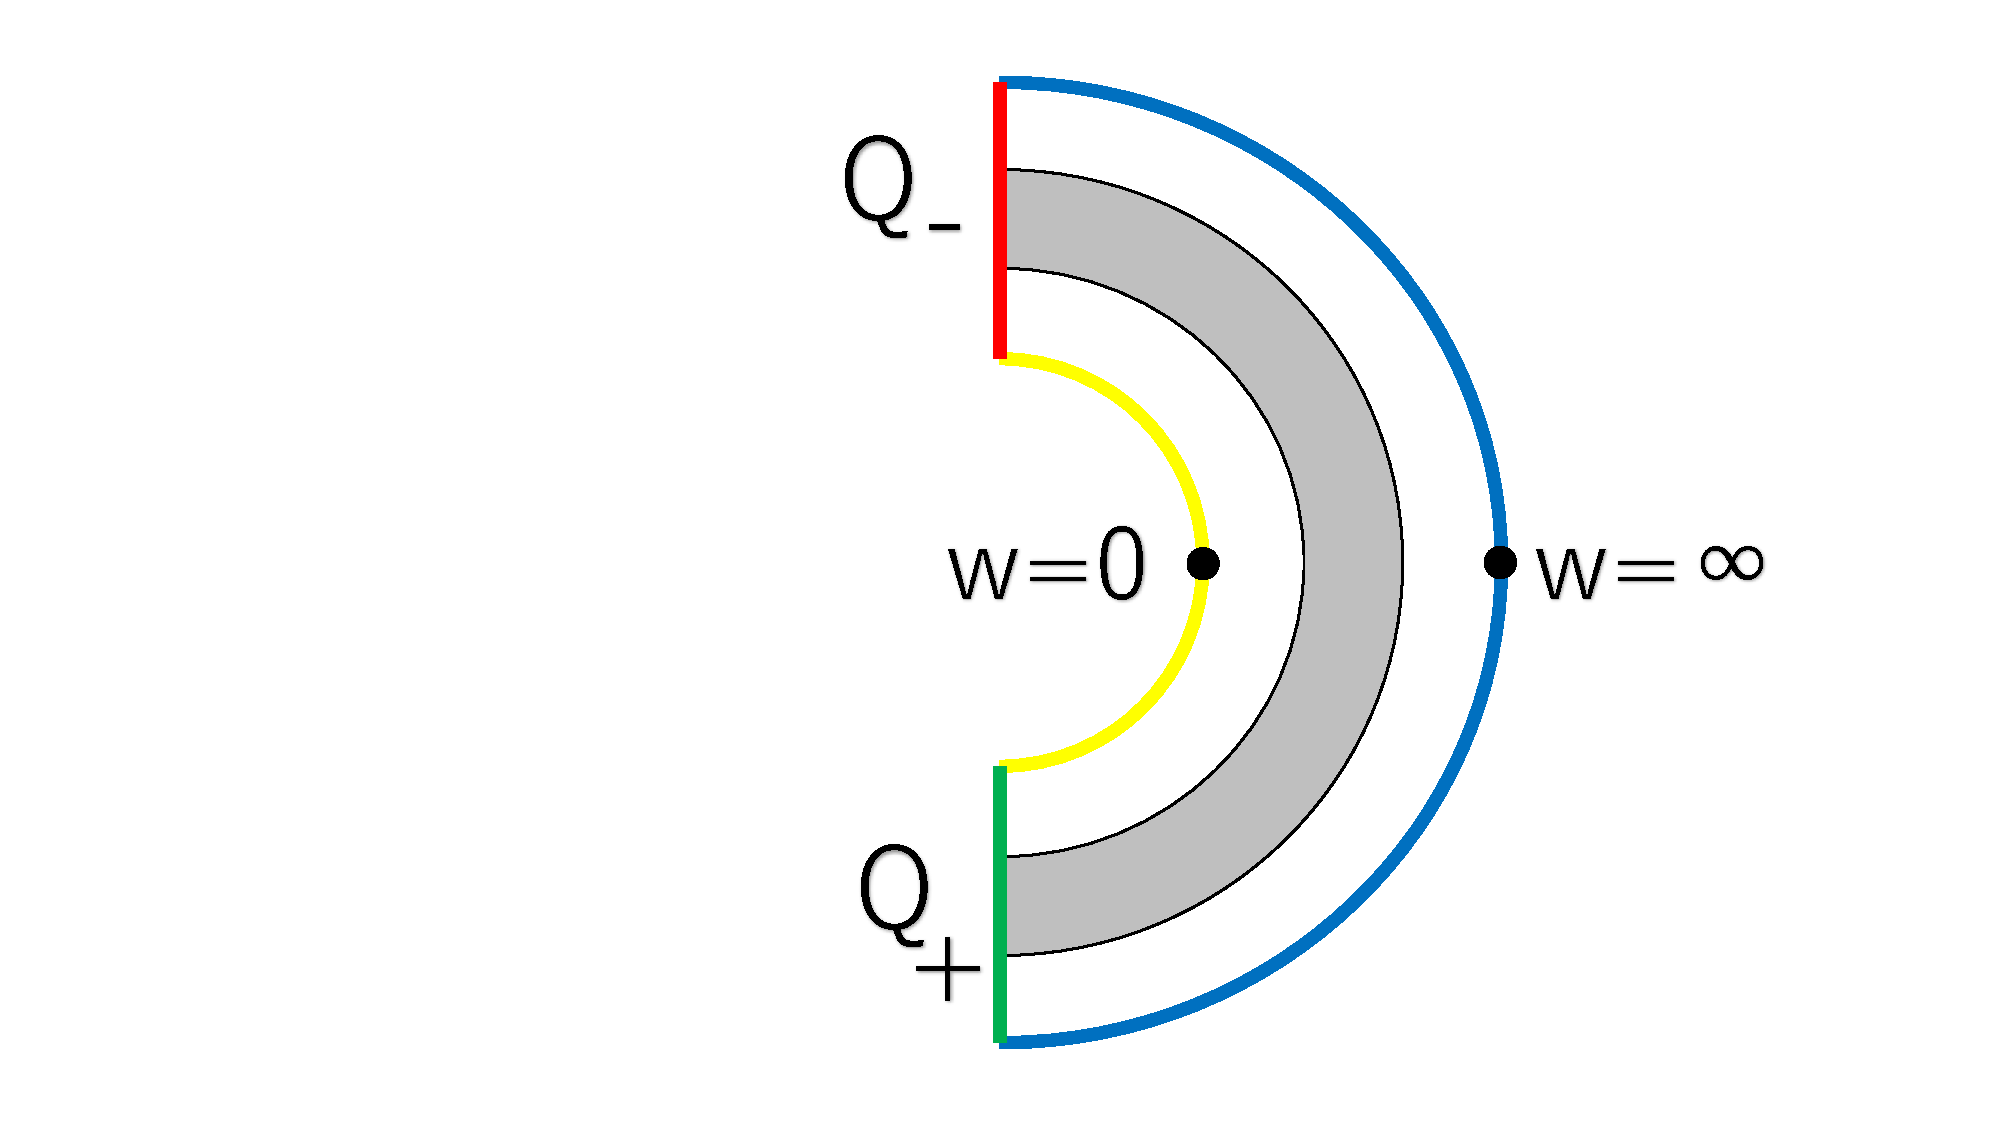
\includegraphics[width=0.7\linewidth]{DQads.pdf}
	\caption{双対なBTZ時空の$\tau=0$の図。この面で測地線を見つければよい。}
	\label{fig:dqads}
\end{figure}

いま、$w$座標での区間$A=[x_1,x_2]$の真空のエンタングルメントエントロピーを笠-高柳公式から求める。$w_i=x_i+i\tau_i\ (i=1,2)$に対応する$\nu,\zeta$座標の点を$\nu_i,\zeta_i$とする。

$c\gg 1$近似を使えば、エンタングルメントエントロピーは
\begin{align}
S_A=\min\{ S_A^{con},S_A^{dis} \}
\end{align}
として求まる。ただし$S_A^{con}$は$\zeta_1,\zeta_2$を結ぶ測地線の長さで決まる。non-rotating BTZ空間の境界の$2$点間の測地線の長さは(\ref{geodlengthGlobal})において$L=\beta^{-1}$として$\sin$を$\sinh$と読み替えればよいから、$S_A^{con}$は
\begin{align}
S^{con}_A&=\frac{c}{6}\log \left( \frac{4\beta^2}{\delta_1\delta_2}\sinh\left(\frac{\zeta_1-\zeta_2}{2\beta} \right)\sinh\left(\frac{\overline{\zeta}_1-\overline{\zeta}_2}{2\beta} \right) \right)\\
&=\frac{c}{6}\log \left( \left(\frac{1}{\pi\epsilon}\right)^2\left|\frac{dw_1}{d\nu_1}\right|\left|\frac{dw_2}{d\nu_2}\right|\sin\left(\pi (\nu_1-\nu_2) \right)\sin\left(\pi (\overline{\nu}_1-\overline{\nu}_2) \right) \right)
\end{align}
となる。ただし$\delta_i (i=1,2)$は\ref{cutofftransf}と同様に、
\begin{align}
\epsilon = \frac{1}{2\pi\beta}\left|\frac{dw_i}{d\nu_i}\right| \delta_i
\end{align}
で関係している。

また$S_A^{dis}$は$\zeta_1,\zeta_2$とそれぞれの鏡像点を結ぶ測地線の長さとして決まる。ただし今の場合、boundary surfaceが2つあるので、ホモロジー条件に注意する必要がある。BCFTの境界$[-b-ia,-b+ia],[b-ia,b+ia]$に対応するboundary surfaceをそれぞれ$Q_-,Q_+$を呼ぶことにする。$\zeta_1,\zeta_2$が共に$Q_+$にエンドする場合や、共に$Q_-$にエンドする場合にはそのまま測地線の長さがエントロピーになる。しかし$\zeta_1,\zeta_2$がそれぞれ別の$Q_{\pm}$にエンドする場合、ホモロジー条件からBTZ BHのエントロピーの半分だけ新たに寄与が生じる。
\begin{figure}[h]
	\centering
	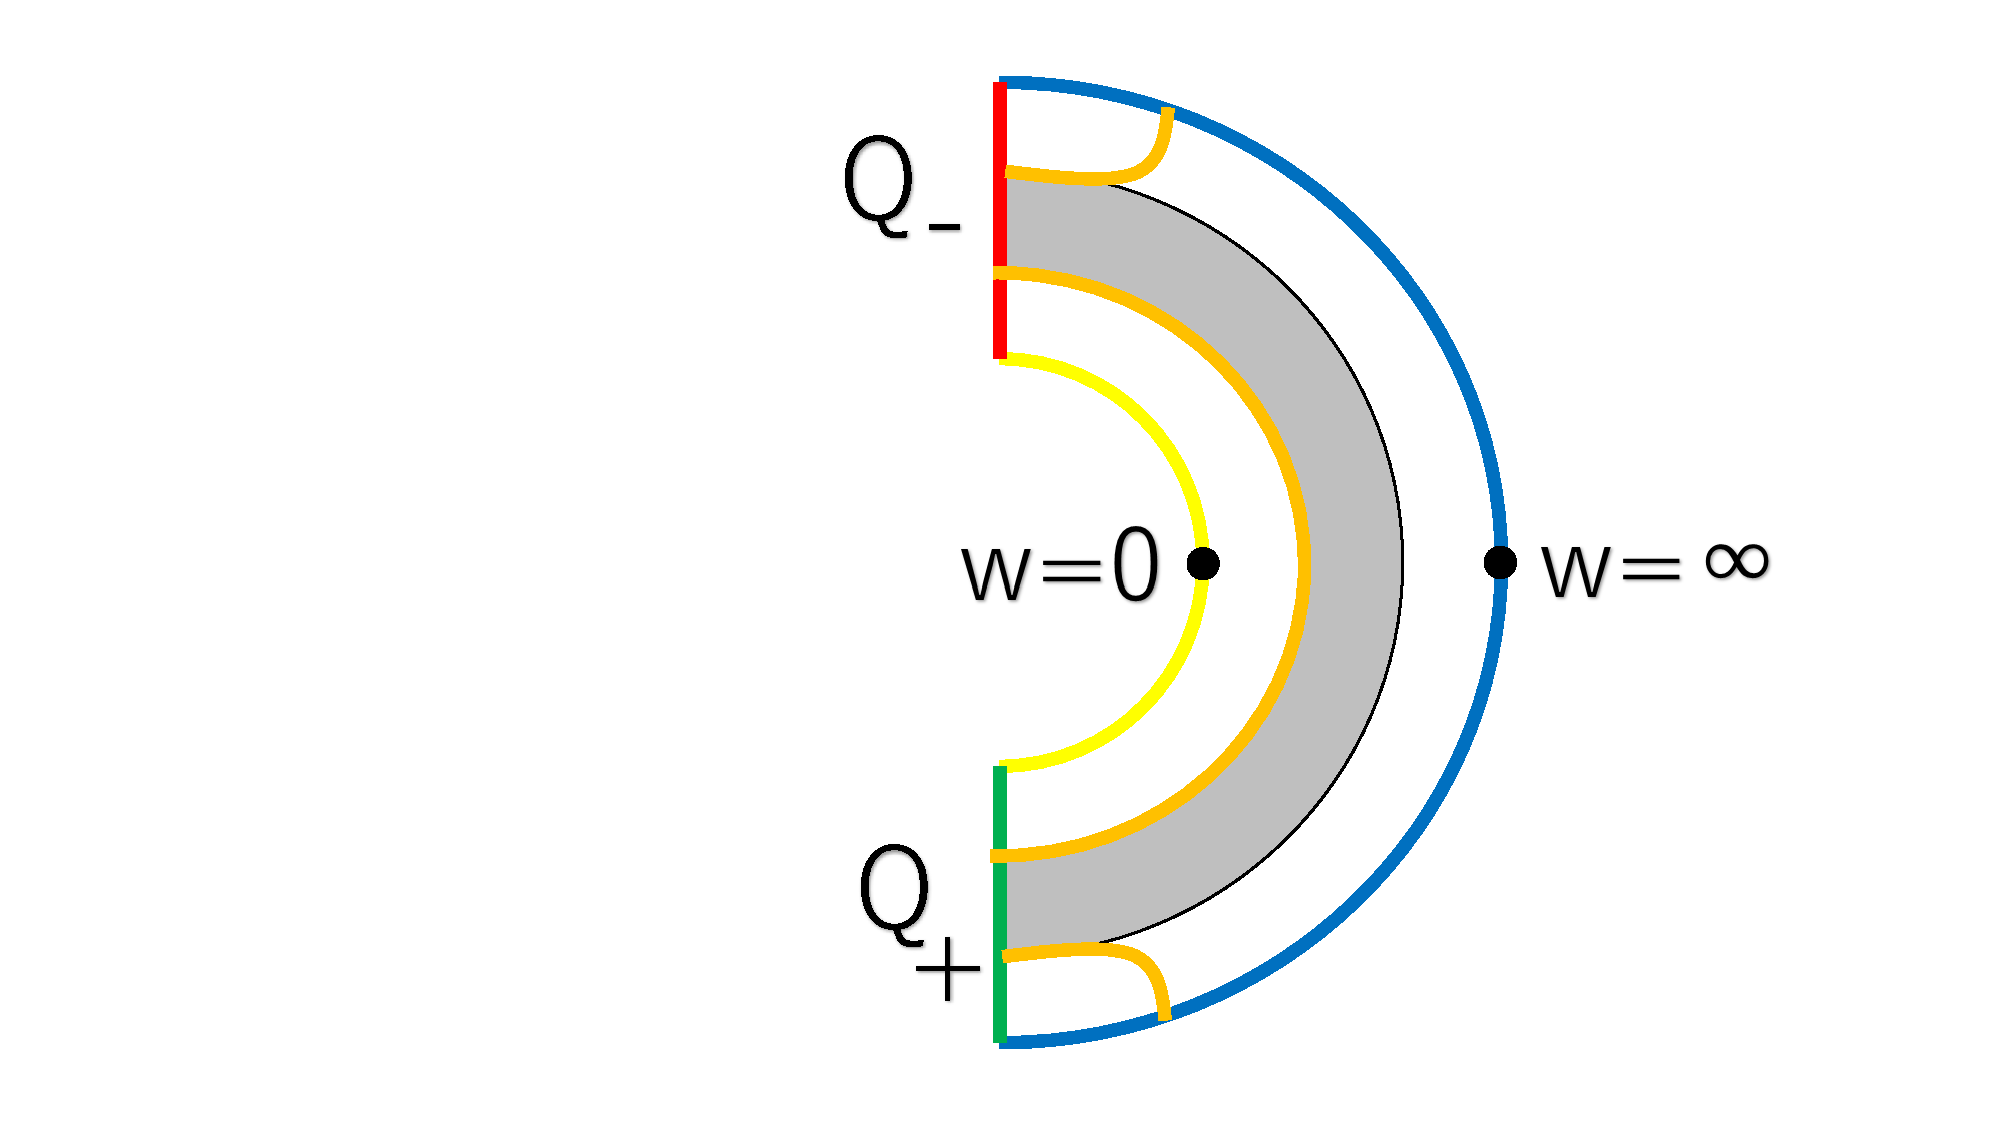
\includegraphics[width=0.7\linewidth]{DQadsgeod.pdf}
	\caption{たとえば連結区間$A=[x_1,x_2],\ x_1\lesssim -b<b\lesssim x_2$についてのEEを考える。これに双対なAdSのセットアップを考えると中央の領域と外側の領域が離れたところにある。このときホモロジー条件により中央の領域の部分からブラックホールエントロピーの半分の値が現れる。}
	\label{fig:dqadsgeod}
\end{figure}

つまり$S_A^{dis}$は以下の式で求められる。

\begin{align}
S_A^{dis}=\min_{\sigma_1=\pm 1,\sigma_2=\pm 1}&\left( \frac{c}{6}\log \frac{1}{\pi\epsilon}\left|\frac{dw_1}{d\nu_1}\right| \sin\left(\pi(\nu_1-\overline{\nu}_1+\frac{i \sigma_1\beta^{-1}}{2})\right)+(1\leftrightarrow 2)\right.\notag\\
&\left.+\frac{1-\sigma_1\sigma_2}{2}\times \frac{c}{6}\pi\beta^{-1}\right)
\end{align}

\subsub{数値計算}
上の計算を数値計算したものがグラフ\ref{fig:dh528}である。$b=50,a=0.05$で計算しており、左上図は部分系$[100,200]$、右上図は部分系$[10,30]$、左下図は部分系$[30,100]$、右下図は$[-150,100]$にとった場合である。
\begin{figure}[H]
	\centering
	\begin{tabular}{c}
		\begin{minipage}{0.50\hsize}
			\centering
			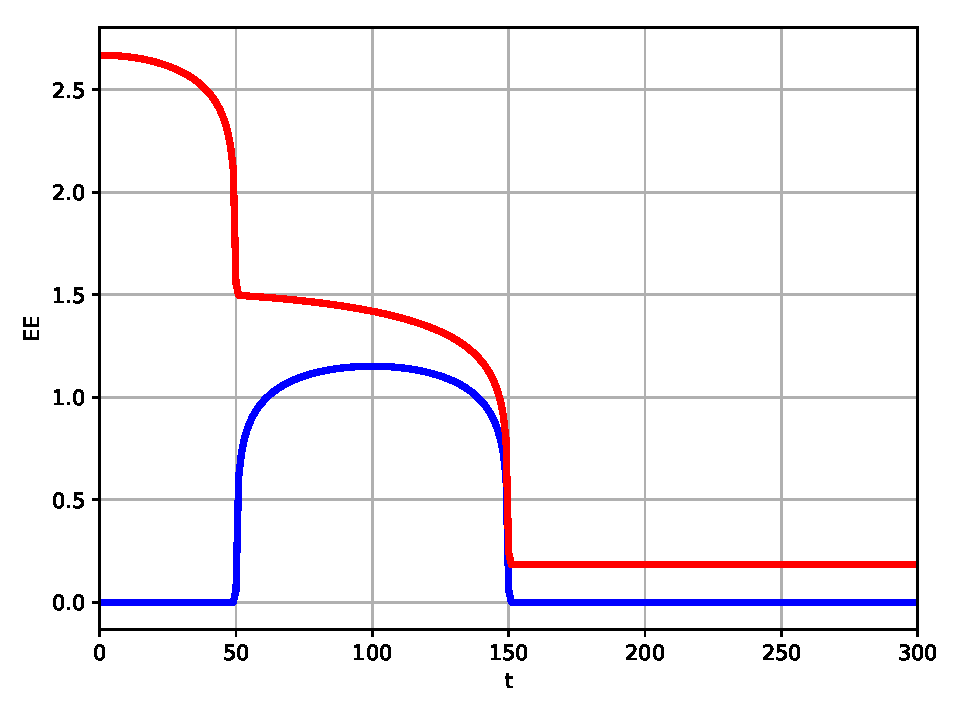
\includegraphics[width=\linewidth]{dh528_100_200.pdf}
		\end{minipage}
		\begin{minipage}{0.50\hsize}
			\centering
			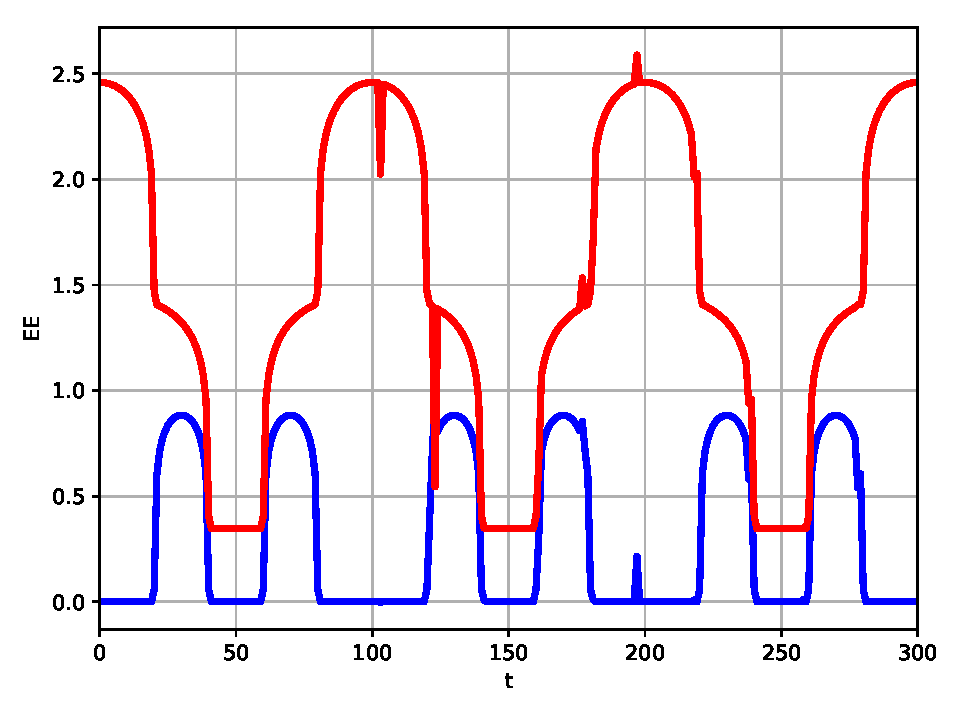
\includegraphics[width=\linewidth]{dh528_10_30.pdf}
		\end{minipage}
		\begin{minipage}{0.06\hsize}
			\vspace{10mm}
		\end{minipage} \\
		\begin{minipage}{0.50\hsize}
			\centering
			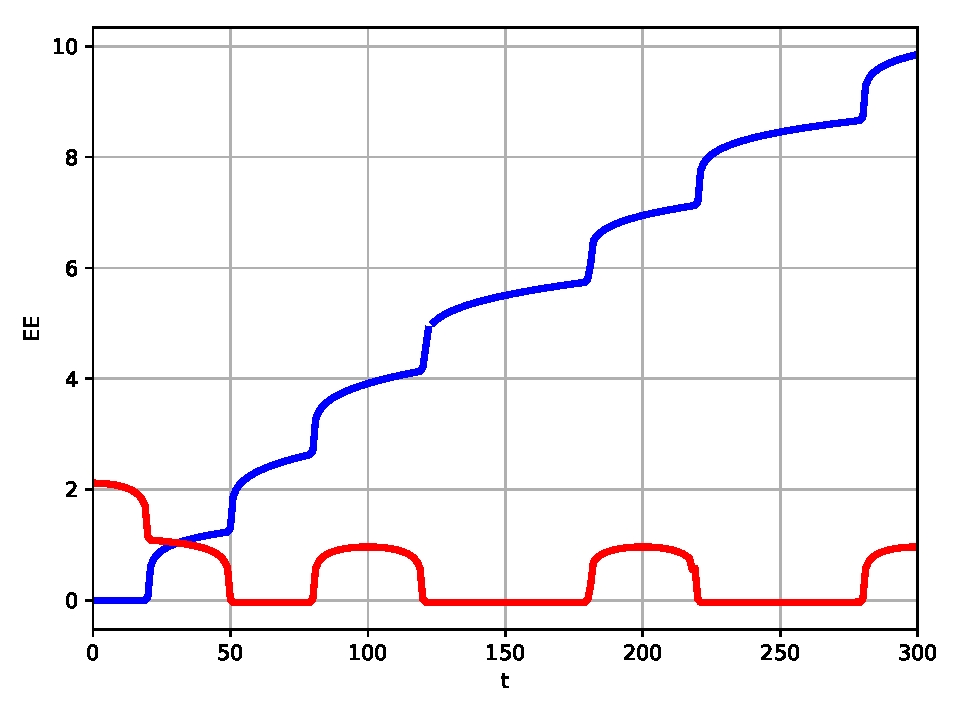
\includegraphics[width=\linewidth]{dh528_30_100.pdf}
		\end{minipage}
		\begin{minipage}{0.50\hsize}
			\centering
			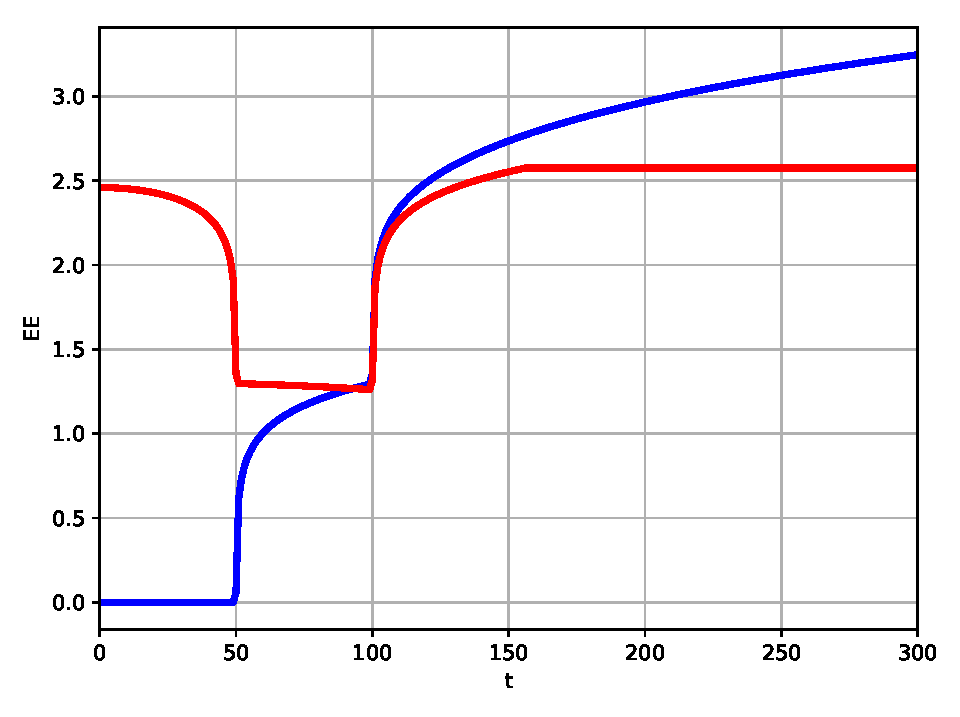
\includegraphics[width=\linewidth]{dh528_150_100.pdf}
		\end{minipage}
	\end{tabular}
	\caption{重力双対を持つ共形場理論の真空を$b=50,a=0.05$で2重分離クエンチしたときのEEのグラフ。横軸は時間$t$で、縦軸は真空の寄与を引いたEE $S_A(t)-S_\text{vac}$をプロットしている。}
	\label{fig:dh528}
\end{figure}
この結果から、右下の図を除いて準粒子描像に当てはまっていることが分かる。

\subsub{BTZ相での、中央の領域$C$を囲む領域のEE}
中央の領域$C$を覆う領域$A,\ (C\subset A)$に対する$S_A(t)-S_\text{vac}$はDirac場の時とは異なり、$t\to\infty$極限をとらなくてもエントロピーはある値に到達した後で一定値になる。これは重力双対をもつような共形場理論がDirac場に比べて非常にカオス性が強く、情報が瞬時に粗視化されてしまうことが表れている。とくに熱力学極限をとればその一定値は、Dirac場と同様に
\begin{align}
S_C(t\gg b)-S_\text{vac} \sim \frac{c}{6}\pi\beta^{-1} \sim \frac{c}{3}\log\frac{4b}{a}
\end{align}
となる。重力双対をもつ共形場理論の場合でも、$C$の熱力学的エントロピーは$a/2$を紫外カットオフと思った領域$C$のエンタングルメントエントロピーに一致している。

\subsection{thermal AdS ($\beta>1$)の場合}
\subsub{解析計算}
逆温度$\beta$のthermal AdSは逆温度$\beta^{-1}$のthermal non-rotating BTZに等しいことに注意すると、$\zeta$座標のCFTに対するthermal AdSの計量は
\begin{align}
ds^2&=\frac{1}{z^2}\left( \frac{dz^2}{1-\beta^2z^2}+\left(1-\beta^2z^2\right)dX^2+dT^2 \right)\\
X&\sim X+2\pi/\beta,\ T\sim T+2\pi
\end{align}
となる。

したがってThermal AdS相での$S_A^{con}$は
\begin{align}
S^{con}_A&=\frac{c}{6}\log \left( \frac{4}{\beta^2\delta_1\delta_2}\sinh\left(\frac{\beta(\zeta_1-\zeta_2)}{2} \right)\sinh\left(\frac{\beta(\overline{\zeta}_1-\overline{\zeta}_2)}{2} \right) \right)\\
&=\frac{c}{6}\log \left( \left(\frac{1}{\pi\beta\epsilon}\right)^2\left|\frac{dw_{1}}{d\nu_{1}}\right|\left|\frac{dw_{2}}{d\nu_{2}}\right|\sin\left(\pi\beta (\nu_1-\nu_2) \right)\sin\left(\pi\beta (\overline{\nu}_1-\overline{\nu}_2) \right)\right)
\end{align}
また$S^{dis}_A$は
\begin{equation}
S^{dis}_A=\min_{\sigma_1,\sigma_2=\pm 1}\left[\frac{c}{6}\log \left( \frac{1}{\pi\beta\epsilon}\left|\frac{dw_{1}}{d\nu_{1}}\right|\sinh\left(\pi\beta\left(\nu_1-\overline{\nu}_1+ \sigma_1 \frac{i}{2\beta}\right)\right)\right)+(1\leftrightarrow 2)\right]
\end{equation}
で計算される。

\subsub{数値計算}
$b=50,a=50$で計算した結果をグラフ\ref{fig:dh0945}にあげる。部分系の取り方は同様で、左上図は部分系$[100,200]$、右上図は部分系$[10,30]$、左下図は部分系$[30,100]$、右下図は$[-150,100]$にとった場合である。
\begin{figure}[H]
	\centering
	\begin{tabular}{c}
		\begin{minipage}{0.50\hsize}
			\centering
			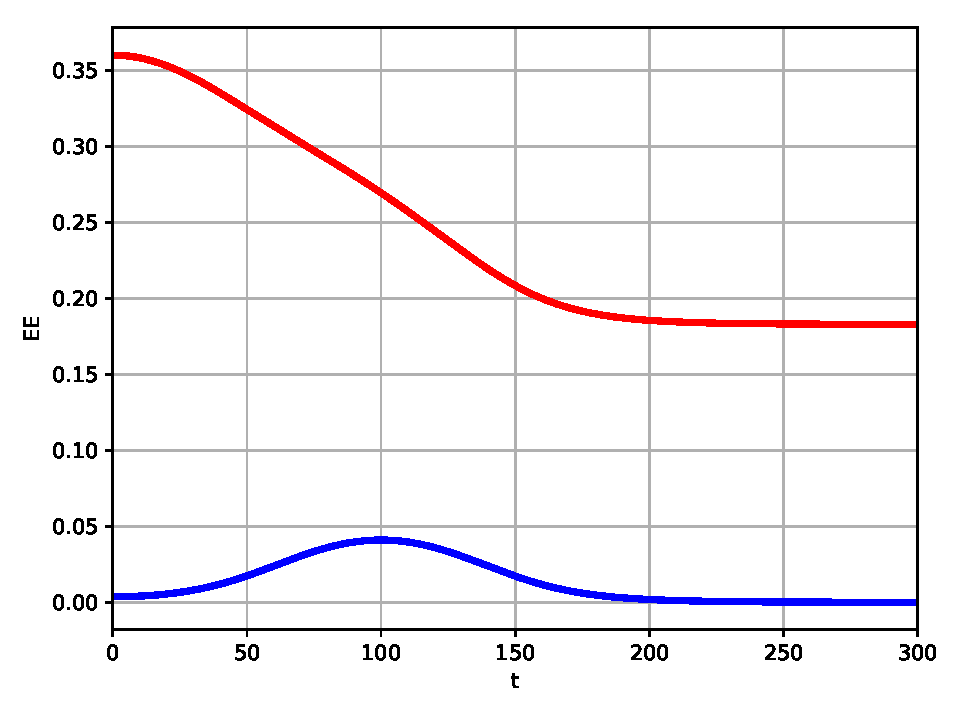
\includegraphics[width=\linewidth]{dh0945_100_200.pdf}
		\end{minipage}
		\begin{minipage}{0.50\hsize}
			\centering
			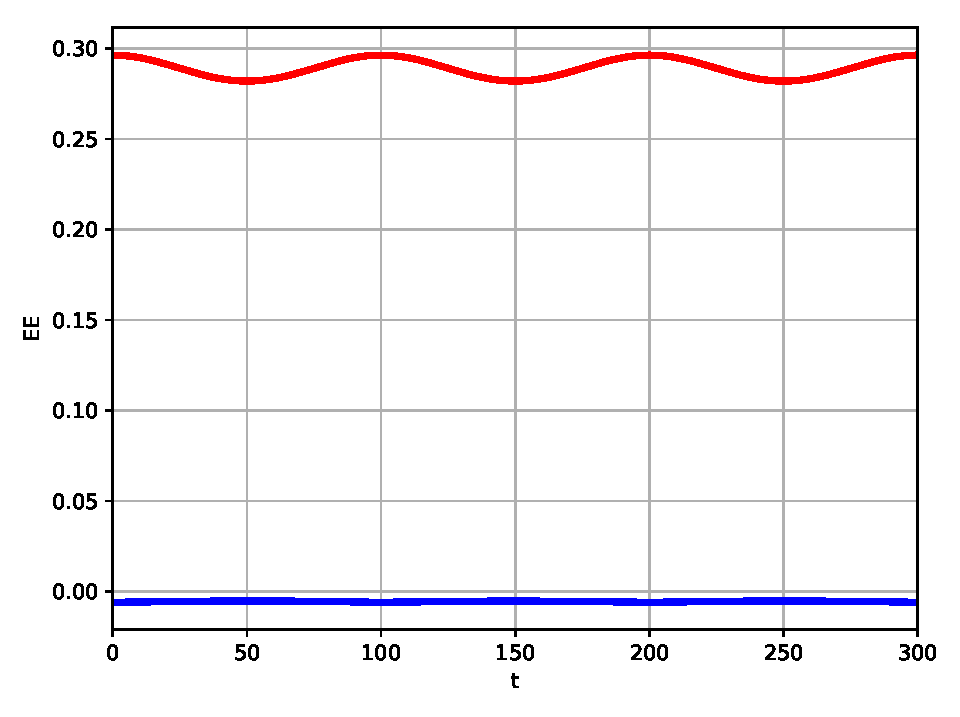
\includegraphics[width=\linewidth]{dh0945_10_30.pdf}
		\end{minipage}
		\begin{minipage}{0.06\hsize}
			\vspace{10mm}
		\end{minipage} \\
		\begin{minipage}{0.50\hsize}
			\centering
			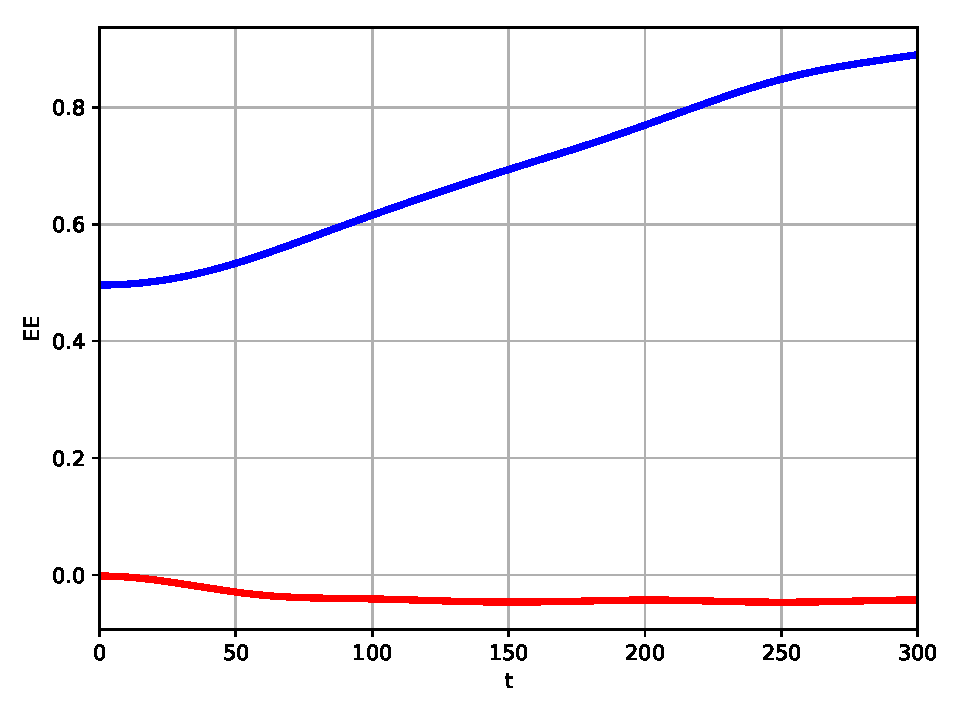
\includegraphics[width=\linewidth]{dh0945_30_100.pdf}
		\end{minipage}
		\begin{minipage}{0.50\hsize}
			\centering
			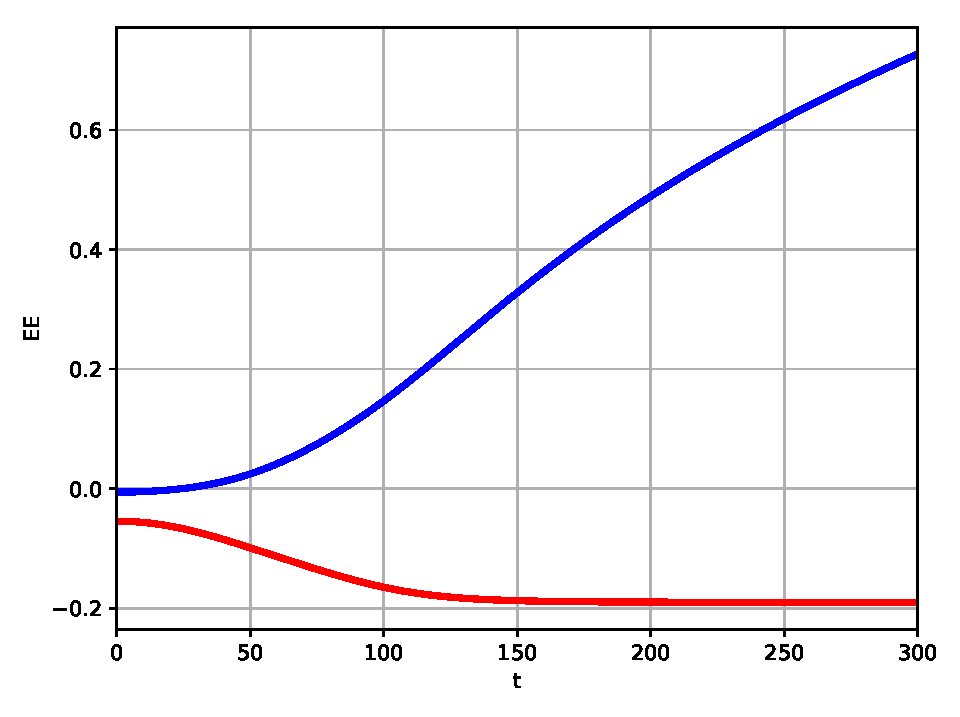
\includegraphics[width=\linewidth]{dh0945_150_100.pdf}
		\end{minipage}
	\end{tabular}
	\caption{重力双対を持つ共形場理論の真空を$b=50,a=50$で2重分離クエンチしたときのEE}
	\label{fig:dh0945}
\end{figure}
この結果から、右下の図を除いて準粒子描像に当てはまっていることが分かる。


\section{2つの1重分離クエンチと2重分離クエンチの比較と重力相互作用}\label{sec:DSQSPQ}

3次元AdS重力はChern-Simons理論だったので、その内部領域には力学的自由度が無い。しかし境界には力学的自由度が存在し、これはboundary gravitonと呼ばれている。

1重クエンチの解析で、共形場理論の境界の双対は、AdS空間での重い物体であることが分かった。我々の2重クエンチのモデルにおいても同様のことが成り立つと考えられるが、このときboundary gravitonによって2つの重い物体同士は引き合うと考えられる。
\begin{figure}[h]
	\centering
	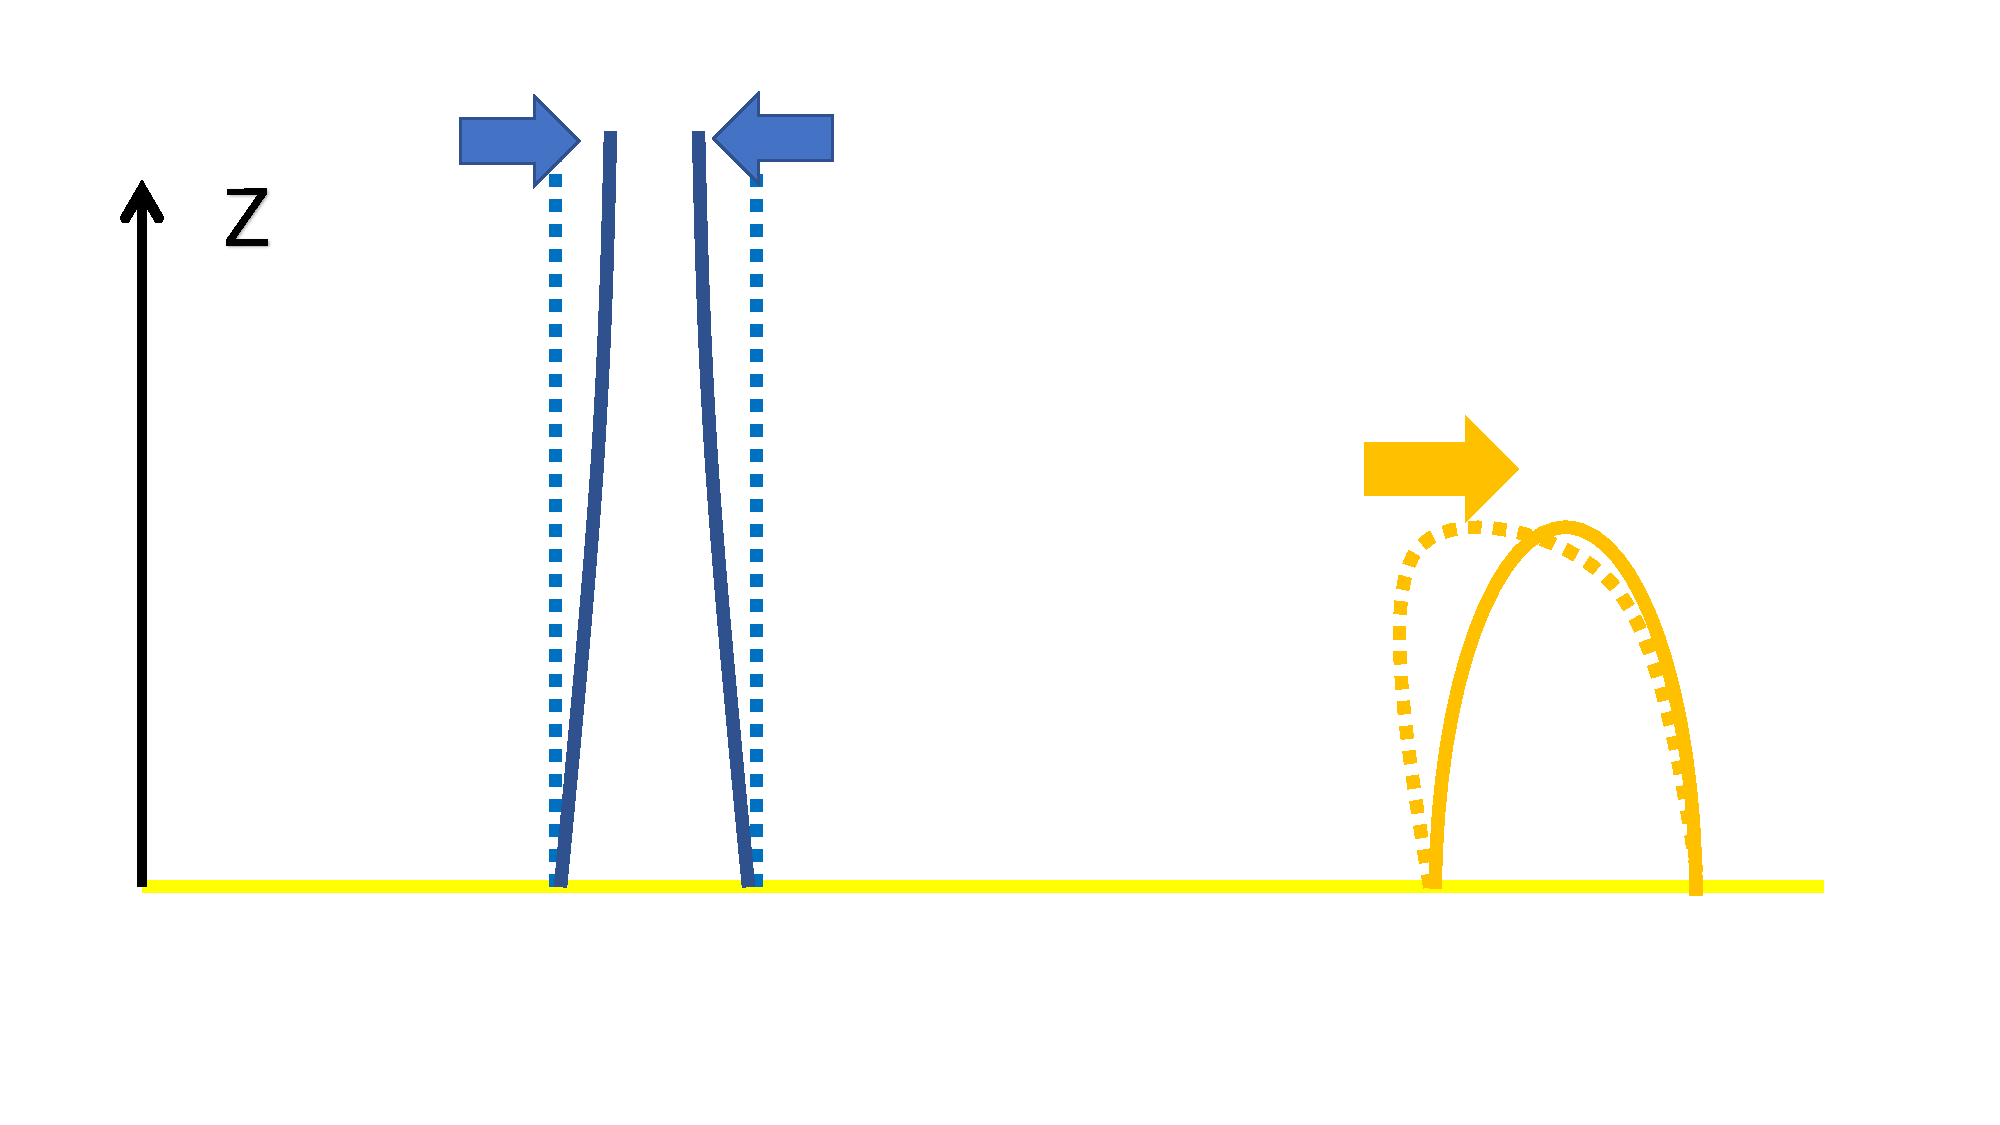
\includegraphics[width=0.7\linewidth]{DQgravdual.pdf}
	\caption{点線が重力相互作用が無いと仮定した場合の境界・測地線の図で、実線が今回のセットアップの図である。}
	\label{fig:dqgravdual}
\end{figure}
このとき笠-高柳公式を考えると、クエンチ点から離れたところの測地線を2重クエンチの場合と、2つの独立な1重クエンチで比較したときに、前者のほうが計量のゆがみが減ることにより短くなると考えられる。そこで次の予想を立てた。
\begin{align}\label{conjecture}
S^\text{double}-(S^{\text{single, }+b}+S^{\text{single, }-b})<S_\text{vac}
\end{align}
ただし$S_\text{vac}=\frac{c}{3}\log\frac{L}{\epsilon}$は真空のエンタングルメントエントロピーを表している。

たとえば$b=50,a=1$で部分系$A=[100,200]$に対して比
\begin{align}
R=\frac{S^\text{double}-S_\text{vac}}{S^{\text{single, }+b}+S^{\text{single, }-b}-2S_\text{vac}}
\end{align}
を計算してみるとグラフのようになり、確かに上の不等式は成り立っている。
\begin{figure}[h]
	\centering
	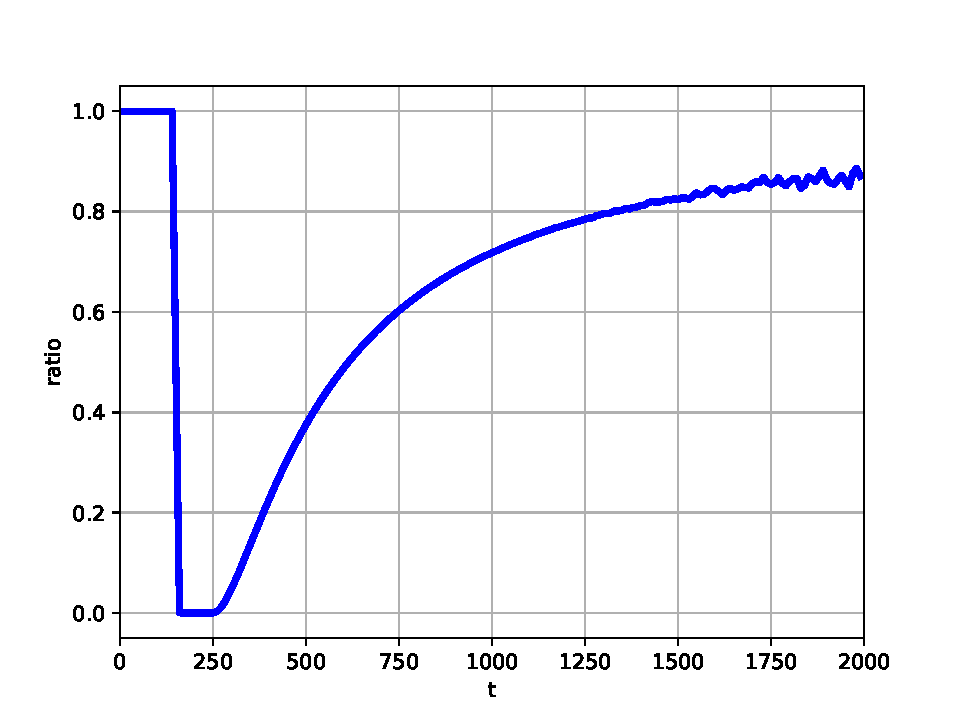
\includegraphics[width=0.7\linewidth]{DSratio.pdf}
	\caption{各時刻$t$での比$R$の値。$R<1$なら\ref{conjecture}が成立している。}
	\label{fig:dsratio}
\end{figure}

$b\ll x_1,x_2$となるような部分系$A=[x_1,x_2]$に対しては、boundary gravitonの存在によって、つねに上の不等式が成り立つと我々は予想している。